\section{Operational environment: Maintenance}\label{section:maintenance}
In industrial, business, and domestic settings, maintenance entails functioning checks, maintaining, repairing,
or replacing necessary devices, equipment,  machinery, building structures, and supporting utilities.
This has evolved over time to encompass a variety of terms that indicate various cost-effective techniques for keeping equipment operating;
these actions might occur before or after a failure~\cite{Misc:maintenance_2016_efnms}. %EFNMS

\paragraph{Types}
The marine and air transportation, offshore structures, industrial plant and facility management industries depend on \ac{mro} including scheduled or preventive paint maintenance programmes to maintain and restore coatings applied
to steel in environments subject to attack from erosion, corrosion and environmental pollution~\cite{Report:iso_2018_paints}.

Architectural conservation employs \ac{mro} to preserve, rehabilitate, restore, or reconstruct historical structures with stone,
brick, glass, metal, and wood which match the original constituent materials where possible, or with suitable polymer technologies when not.
The basic types of maintenance falling under \acs{mro} include:
\begin{itemize}
    \item \textbf{Corrective maintenance}, where equipment is repaired or replaced after wear, malfunction or break down.
    \item \textbf{Preventive maintenance}, where equipment is checked and serviced in a planned manner (in scheduled points in time or continuously).
    \item \textbf{Reinforcement}, where equipment is reinforced and hardened to prevent failure.
\end{itemize}
\begin{figure}[t]
    \centering
    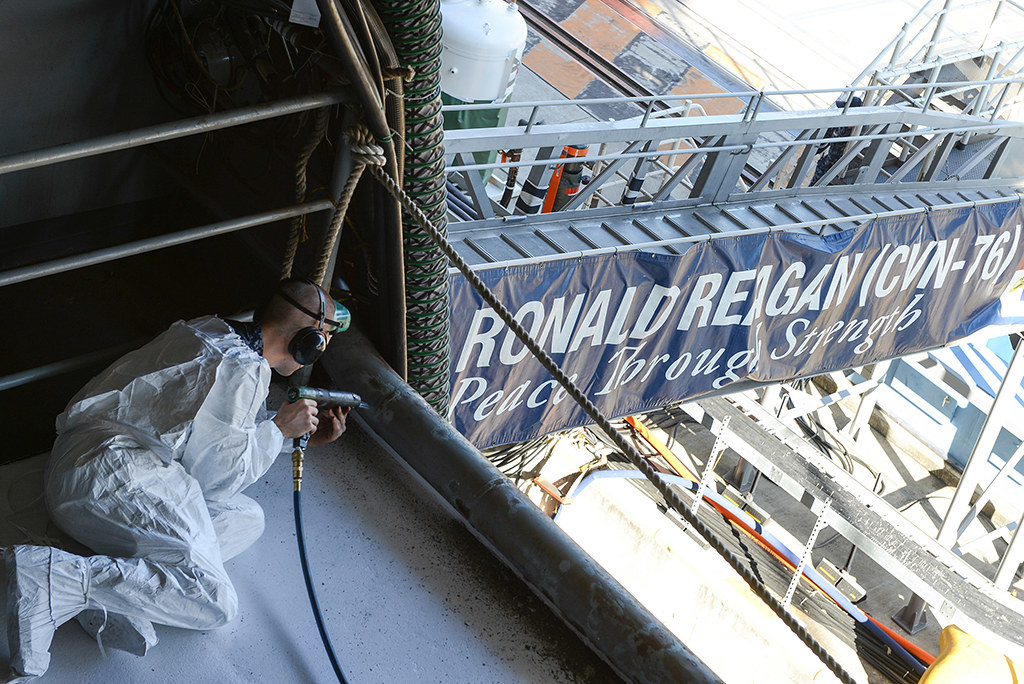
\includegraphics[width=0.8\textwidth]{PM_US_navy.jpg}
    \caption{\citetitle{file:boat_2016_uss} (Source:~\cite{file:boat_2016_uss})}
    \label{fig:boat_us_navy}
\end{figure}
These are huge topics, and we are going to focus mostly on corrective and preventive maintenance.
% \todo{DG:Expand this connection?}

\paragraph{Corrective maintenance} Is a type of reactive maintenance that is performed on equipment after it has broken down or malfunctioned,
sometimes referred to as ``fighting fires''. Not only can wear equipment damage other parts and cause multiple damages, but it can also result in significant repair and
replacement costs as well as lost revenue due to downtime during overhaul. Traditional procedures like welding and metal flame spraying,
as well as designed solutions with thermoset polymeric materials, are used to rebuild and resurface equipment and infrastructure
damaged by erosion and corrosion as part of corrective or preventive maintenance programs.

\subsection{Preventive Maintenance}
\ac{PM} is, according to \citeauthor{Article:nyt_hinds_1985_preventive}~\cite{Article:nyt_hinds_1985_preventive}:
\begin{quote}
    \textit{\dots a routine for periodically inspecting with the goal of noticing small problems and fixing them before major ones develop.}

    % split for better hbox
    \textit{Ideally, nothing breaks down!}
\end{quote}

The main objectives of preventive maintenance are as follows:
\begin{enumerate}
    \item \textbf{Enhance} capital equipment productive life.
    \item \textbf{Reduce} critical equipment breakdown.
    \item \textbf{Minimize} production loss due to equipment failures.
\end{enumerate}
Many people, me included, confuse the phrases \textit{preventive, predictive, and prescriptive} maintenance, and while they are distinct, the latter two might
be considered kinds of preventive maintenance. Preventative maintenance in all forms aids manufacturers in transitioning from a
repair-and-replace to a preventive maintenance approach~\cite{Misc:trout_2019_preventive}. Let's look at the different types of preventative maintenance.

\begin{itemize}
    \item \textbf{\ac{ppm}}, more commonly referred to planned maintenance
          or scheduled maintenance, is any variety of scheduled maintenance to an object or item of equipment. Specifically, planned maintenance is
          a scheduled service visit carried out by a competent and suitable agent, to ensure that an item of equipment is operating correctly and to
          therefore avoid any unscheduled breakdown and downtime. It can be further split in two subcategories:
          \begin{itemize}
              \item \textbf{Calendar-based maintenance} is performed on equipment according to a calendar timetable.
                    In other words, a maintenance activity is triggered by the passage of time.
                    Calendar-based maintenance includes things like: cleaning your air conditioner and replacing the air filter in your heating,
                    ventilation, and air conditioning equipment every three months.

                    When a scheduled task is due, \ac{cmms} are frequently used to keep schedules straight and issue recurring work orders.
              \item \textbf{Usage-based maintenance} uses triggers based on how much each piece of equipment is used.
                    Maintenance managers can create a preventative maintenance schedule based on predefined parameters by tracking usage
                    using equipment monitors and the operating hours of each piece of machinery.

                    For example, when machine $X$ reaches a certain number of hours of operation, this creates a trigger
                    to schedule a booking for a service technician to perform on-demand maintenance.
          \end{itemize}
    \item \textbf{\ac{PdM}} are intended to assist in determining the state of in-service equipment, so that maintenance can be scheduled.
          Because actions are performed only when warranted, this strategy promises cost reductions over routine or time-based preventive maintenance.
          As a result, it is viewed as condition-based maintenance which is carried out in accordance by estimations of an item's degradation status.
          Predictive maintenance's key benefit is that it allows for easy scheduling of corrective maintenance and prevents unexpected equipment breakdowns~\cite{Misc:danielpenn_2020_what}.

          It is particularly useful when coupled with \acs{cmms} software; Logging work requirements data allows managers to review data and notice failure patterns over time.
          This information allows predicting when outages will occur based on historical data and plan maintenance tasks to avoid them~\cite{Misc:trout_2019_preventive}.
    \item \textbf{\ac{cbm}} to put it succinctly, is \textit{maintenance when it is needed}. Although being chronologically much older,
          it is considered one sector or practice within the broader and younger predictive maintenance field, where new \ac{AI} technology and \ac{IoT}
          connectivity abilities are put to use, to help schedule preventive maintenance tasks.
          \acs{cbm} is performed after one or more indicators show that equipment is going to fail or that equipment performance is deteriorating;
          this concept is applicable to both mission-critical systems that incorporate active redundancy and fault reporting, and non-mission-critical systems
          that have a more limited budget; let's explore this in a little more detail.
\end{itemize}

\subsection{Condition-based maintenance \& monitoring}
\begin{figure}[ht]
    \centering
    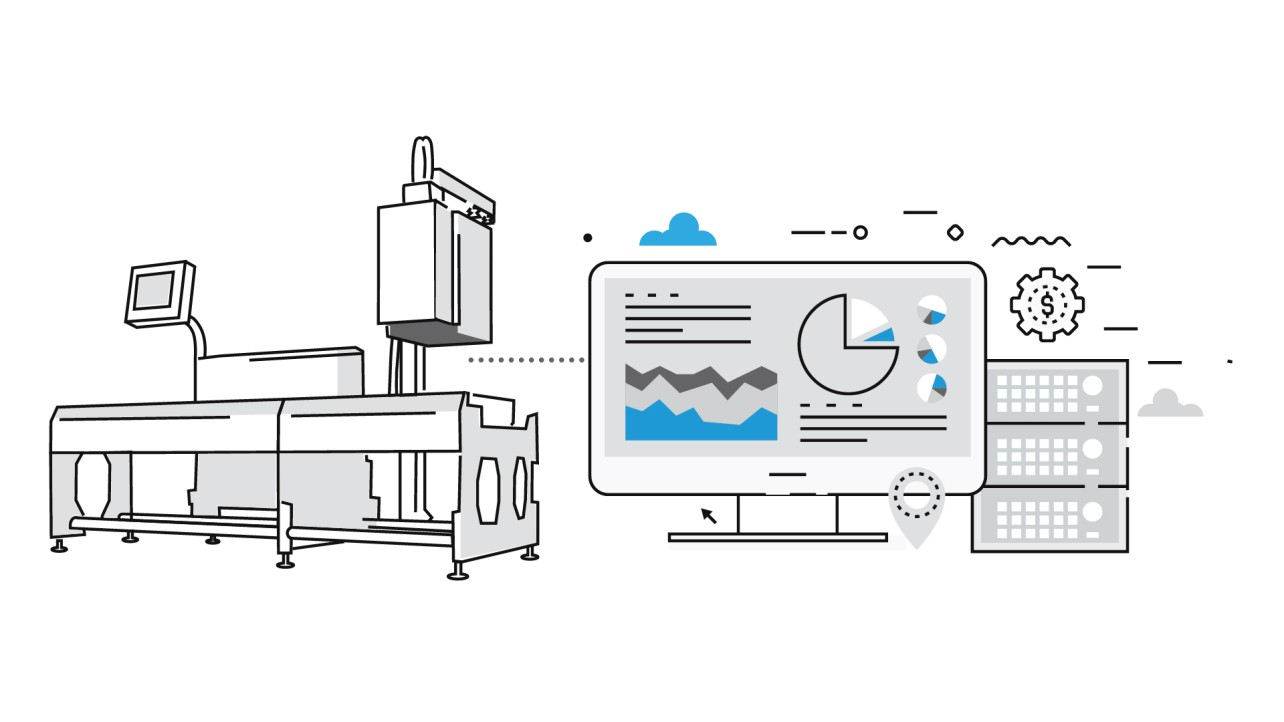
\includegraphics[width=\textwidth]{bizerba_whitepaper.jpg}
    \caption{\acl{cbm} schema (Source:~\cite{file:bizerbaspa_conditionbased})}
\end{figure}
\ac{cbm} was developed to ensure that the proper equipment was maintained at the right time. It is focused on prioritizing and optimizing
maintenance resources using real-time data, through \ac{cm}, which is the process of observing the system's state; how?
Through monitoring parameter(s) of condition in machinery (vibration, voltage, temperature etc.), in order to identify a significant change which is indicative of a developing fault~\cite{Inbook:hitchcock_2012_iso}.
The equipment's health will be determined by this system, and maintenance will be performed only when it is genuinely required.

Recent technological advancements have enabled widespread equipment instrumentation, and, when combined with improved tools for analysing condition data,
maintenance personnel is more than ever able to determine when it is appropriate to undertake maintenance on a piece of equipment.
\ac{cbm}, in essence, should allow maintenance professionals to focus on only the necessary tasks, reducing spare parts costs, system downtime, and maintenance time.
Furthermore, using \ac{ML} based scheduled maintenance could not only predict a possible failure, but also attempts to make result-oriented maintenance recommendations based on that machine's analysis.

\paragraph{Challenges}
Despite its usefulness, there are several challenges to the use of \acl{cbm}.
\begin{enumerate}
    \item First and most important of all, the initial cost can be high since it requires improved instrumentation of the equipment.
          Often the cost of sufficient instruments can be quite large, especially on equipment that is already installed, even though
          wireless systems have reduced the initial cost. Therefore, it is important for the installer to decide the importance of the investment before adding \ac*{cbm} to the equipment.

          For instance, a result of this cost is that the first generation of \ac*{cbm} in the oil and gas industry has only focused on vibration in heavy rotating equipment~\cite{Misc:dida_2020_manufacturing}.
    \item Secondly, introducing this process will invoke a major change in how maintenance is performed, and potentially to the whole maintenance organization in a company.
          As we well know organizational changes are in general difficult.
    \item Lastly, the technical side of it is \textbf{not} simple! Even if some types of equipment can easily be observed by measuring simple
          values such as vibration (displacement, velocity or acceleration), temperature or pressure, it is not trivial to turn this measured data
          into actionable knowledge about the health of the equipment.
\end{enumerate}

\paragraph{Advantages and disadvantages}
\acl{cbm} has some advantages and disadvantages over \acl{ppm}:
\begin{table}[!h]
    \begin{tabularx}{\textwidth}{>{\parskip1ex}X@{\kern4\tabcolsep}>{\parskip1ex}X}
        \toprule
        \hfil\bfseries Pros
         &
        \hfil\bfseries Cons
        \\\cmidrule(r{3\tabcolsep}){1-1}\cmidrule(l{-\tabcolsep}){2-2}
        %% PROS, separated by empty line or \par
        Improved system reliability\par
        Decreased maintenance costs\par
        Decreased number of maintenance operations causes a reduction of human error influences\par
         &
        %% CONS, separated by empty line or \par
        High installation costs, for minor equipment items often more than the value of the equipment\par
        Unpredictable maintenance periods cause costs to be divided unequally\par
        Increased number of parts (the \acs{cbm} installation itself) that need maintenance and checking\par
        \\\bottomrule
    \end{tabularx}
    % \caption{Pros and cons of \acs{cbm}}
\end{table}

% \subsubsection{Repair minimization}
\subsection{A possible solution}
Today, most often, technical data sheets coupled with the knowledge of a number of unique experienced individuals are used to determine when the asset requires maintenance.
Product quality only becomes an issue when customers start complaining and repairs are done when it is already far too late,
All of these puts tremendous strain on the people responsible for the asset, while it could be avoided
Unexpected shutdowns are costly and very demanding for the workforce involved; a possible solution would be making assets smart in order to increase the availability.
The best way to validate the actual health is by having a continuous look at a broad data set and adding a specific multi-aspect monitoring setup
consisting of different sensor types that follow the behaviour of the asset's general state-of-health~\cite{Misc:zensor_official_website}.

\paragraph{\ac{infra}} 
\begin{figure}[ht]
    \centering
    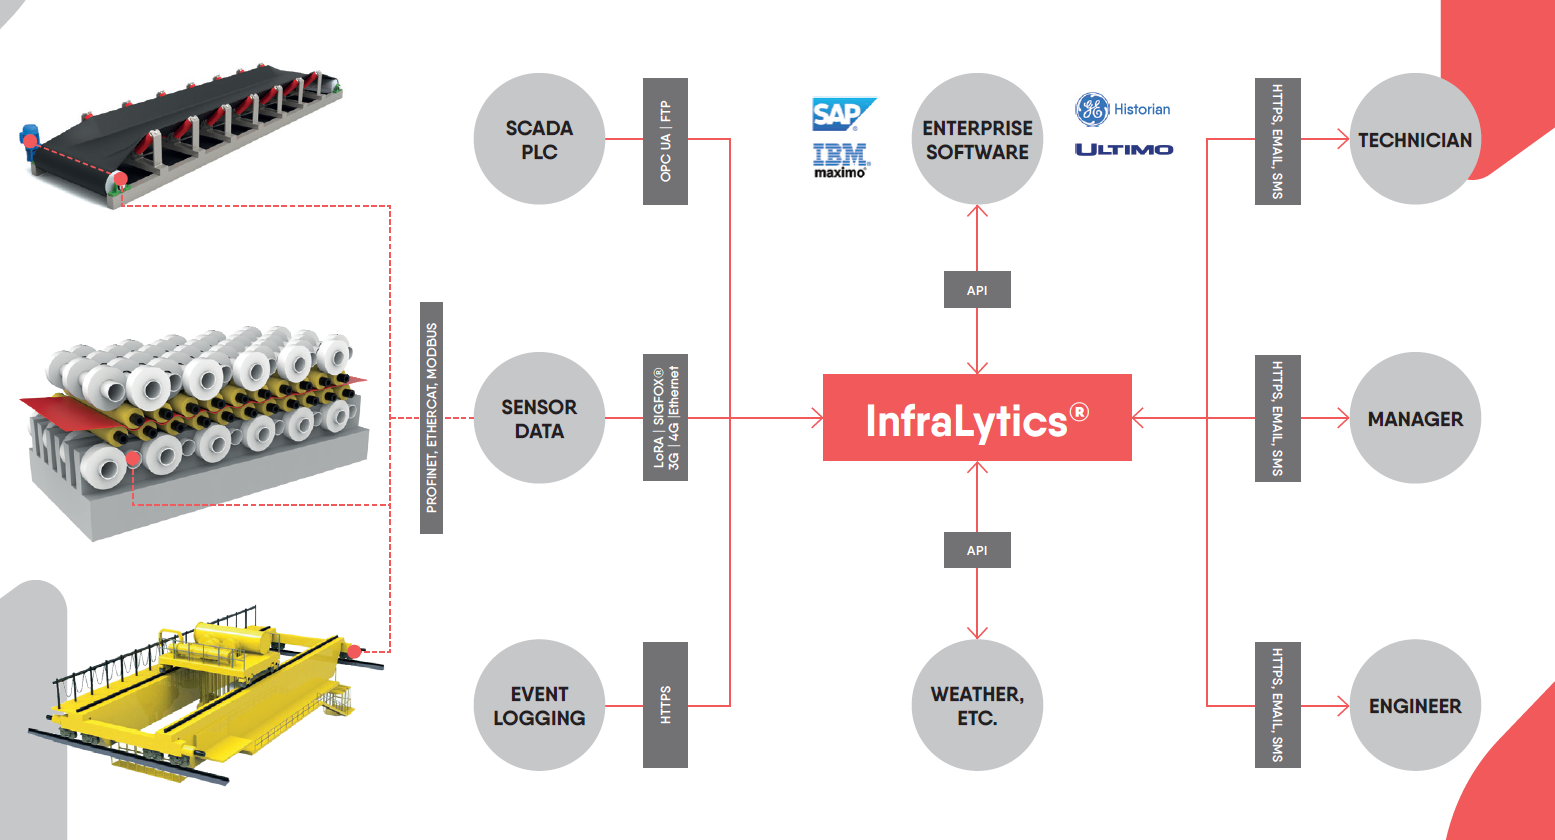
\includegraphics[width=\textwidth]{how_it_works_plan_owner.png}
    \caption{\acl{SaaS} Workflow (Source:~\cite{Misc:zensor_official_website})}
    \label{fig:zensor_flow}
\end{figure}
Zensor platform~\ref{fig:zensor_flow} is designed to make \ac{PdM} as easy as possible. It graphically shows you the current state of your asset, it alarms you when a certain component is about to
break down and the collection and aggregation of all kinds of sensor and operational data makes it possible to go beyond the symptom level of a mechanical failure 
and detect the underlying reason for the breakdown. Relying on \ac{infra} will not only lower your maintenance costs significantly, 
it will also have a serious impact on your plant's efficiency by increasing uptime and lowering the occurrence of unexpected mechanical breakdowns~\cite{Misc:vaningelgem_2020_what}.

